\chapter{Анализ и идентификация физической реализации системы Колпитца}
\label{atu:ch:colpreal}

\section{Отличия реального генератора Колпитца}


Как уже было отмечено,
рассмотренная в разделе \ref{atu:sect:colp} модель
генератора Колпитца, несмотря на её широкое использование
при исследованиях, связанных с хаотической динамикой,
имеет существенные отличия от реального генератора.
Подавляющие большинство элементов достаточно хорошо описываются линейным
приближением. Однако, есть два элемента,
применение линейной модели для которых или же вообще невозможно (транзистор),
или же допустимо при определённых условиях (индуктивность).





\section{Физическая реализация генератора Колпитца и исследование её динамики}

На рис.~\ref{atu:f:colp_schem_real} представлена электрическая схема
реализации генератора Колпитца, используемая в данной работе.
Отличия от схемы, используемой в главе \ref{atu:ch:testsys}
и представленной на рис.~\ref{atu:f:colp_schem}
не принципиальны с точки зрения модели,
и предназначены как для упрощения подключения
измерительных устройств, так и для
обеспечения стабильности определённых потенциалов схемы.

\begin{figure}[htb!]
\centerline{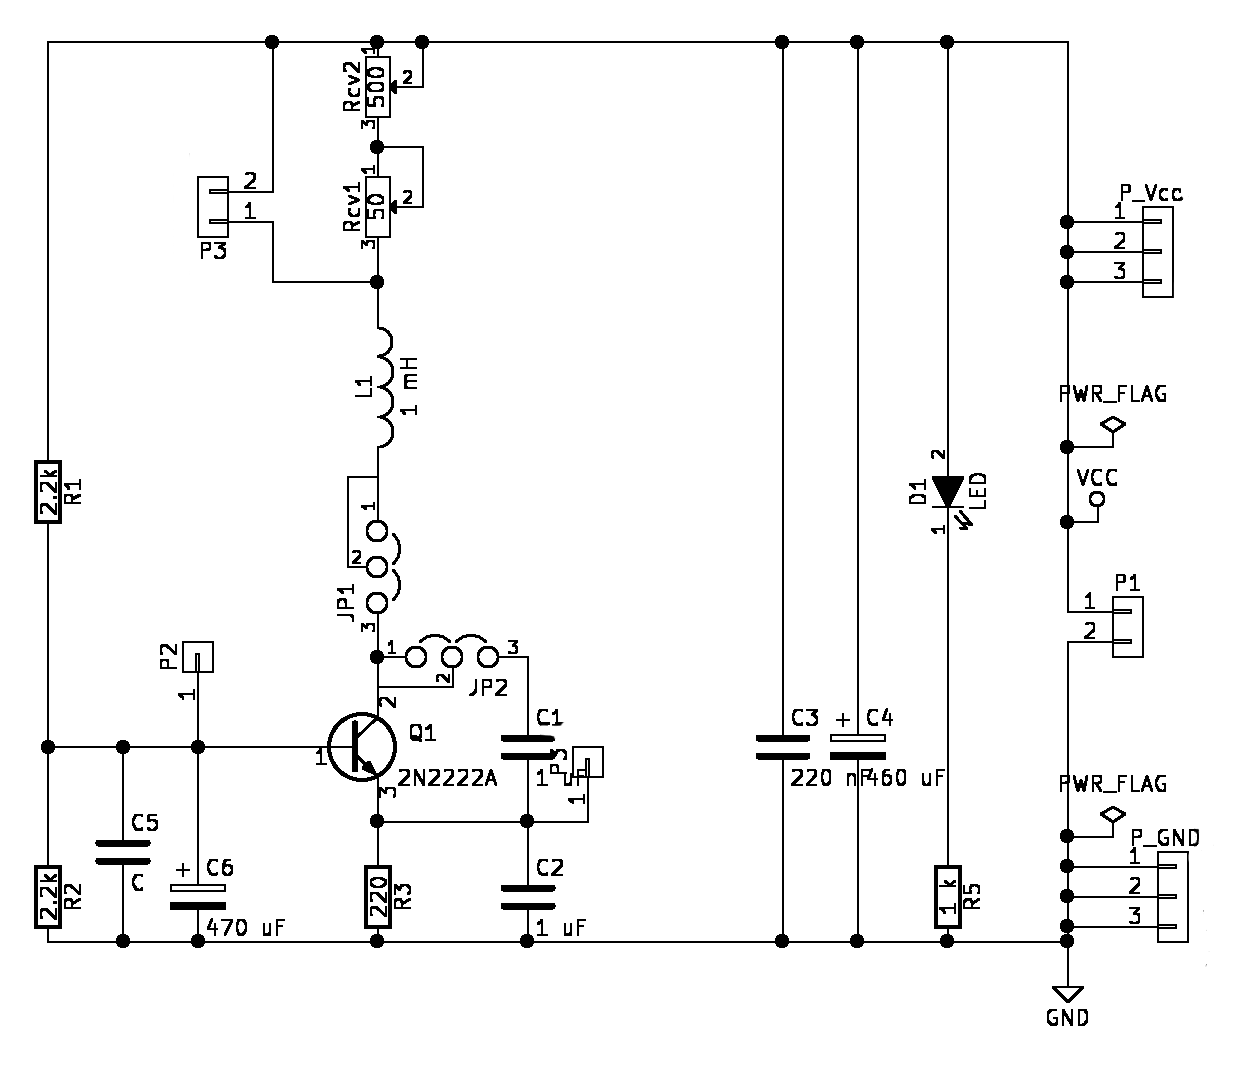
\includegraphics[width=0.8\textwidth]{p/colp_schem_real.png} }
\caption{Электрическая схема реального генератора Колпитца, используемого в данной работе}
\label{atu:f:colp_schem_real}
\end{figure}

Внешний вид cобранной схемы на печатной плате представлен на~(рис.~\ref{atu:f:relax3d_board}).

\begin{figure}[htb!]
\centerline{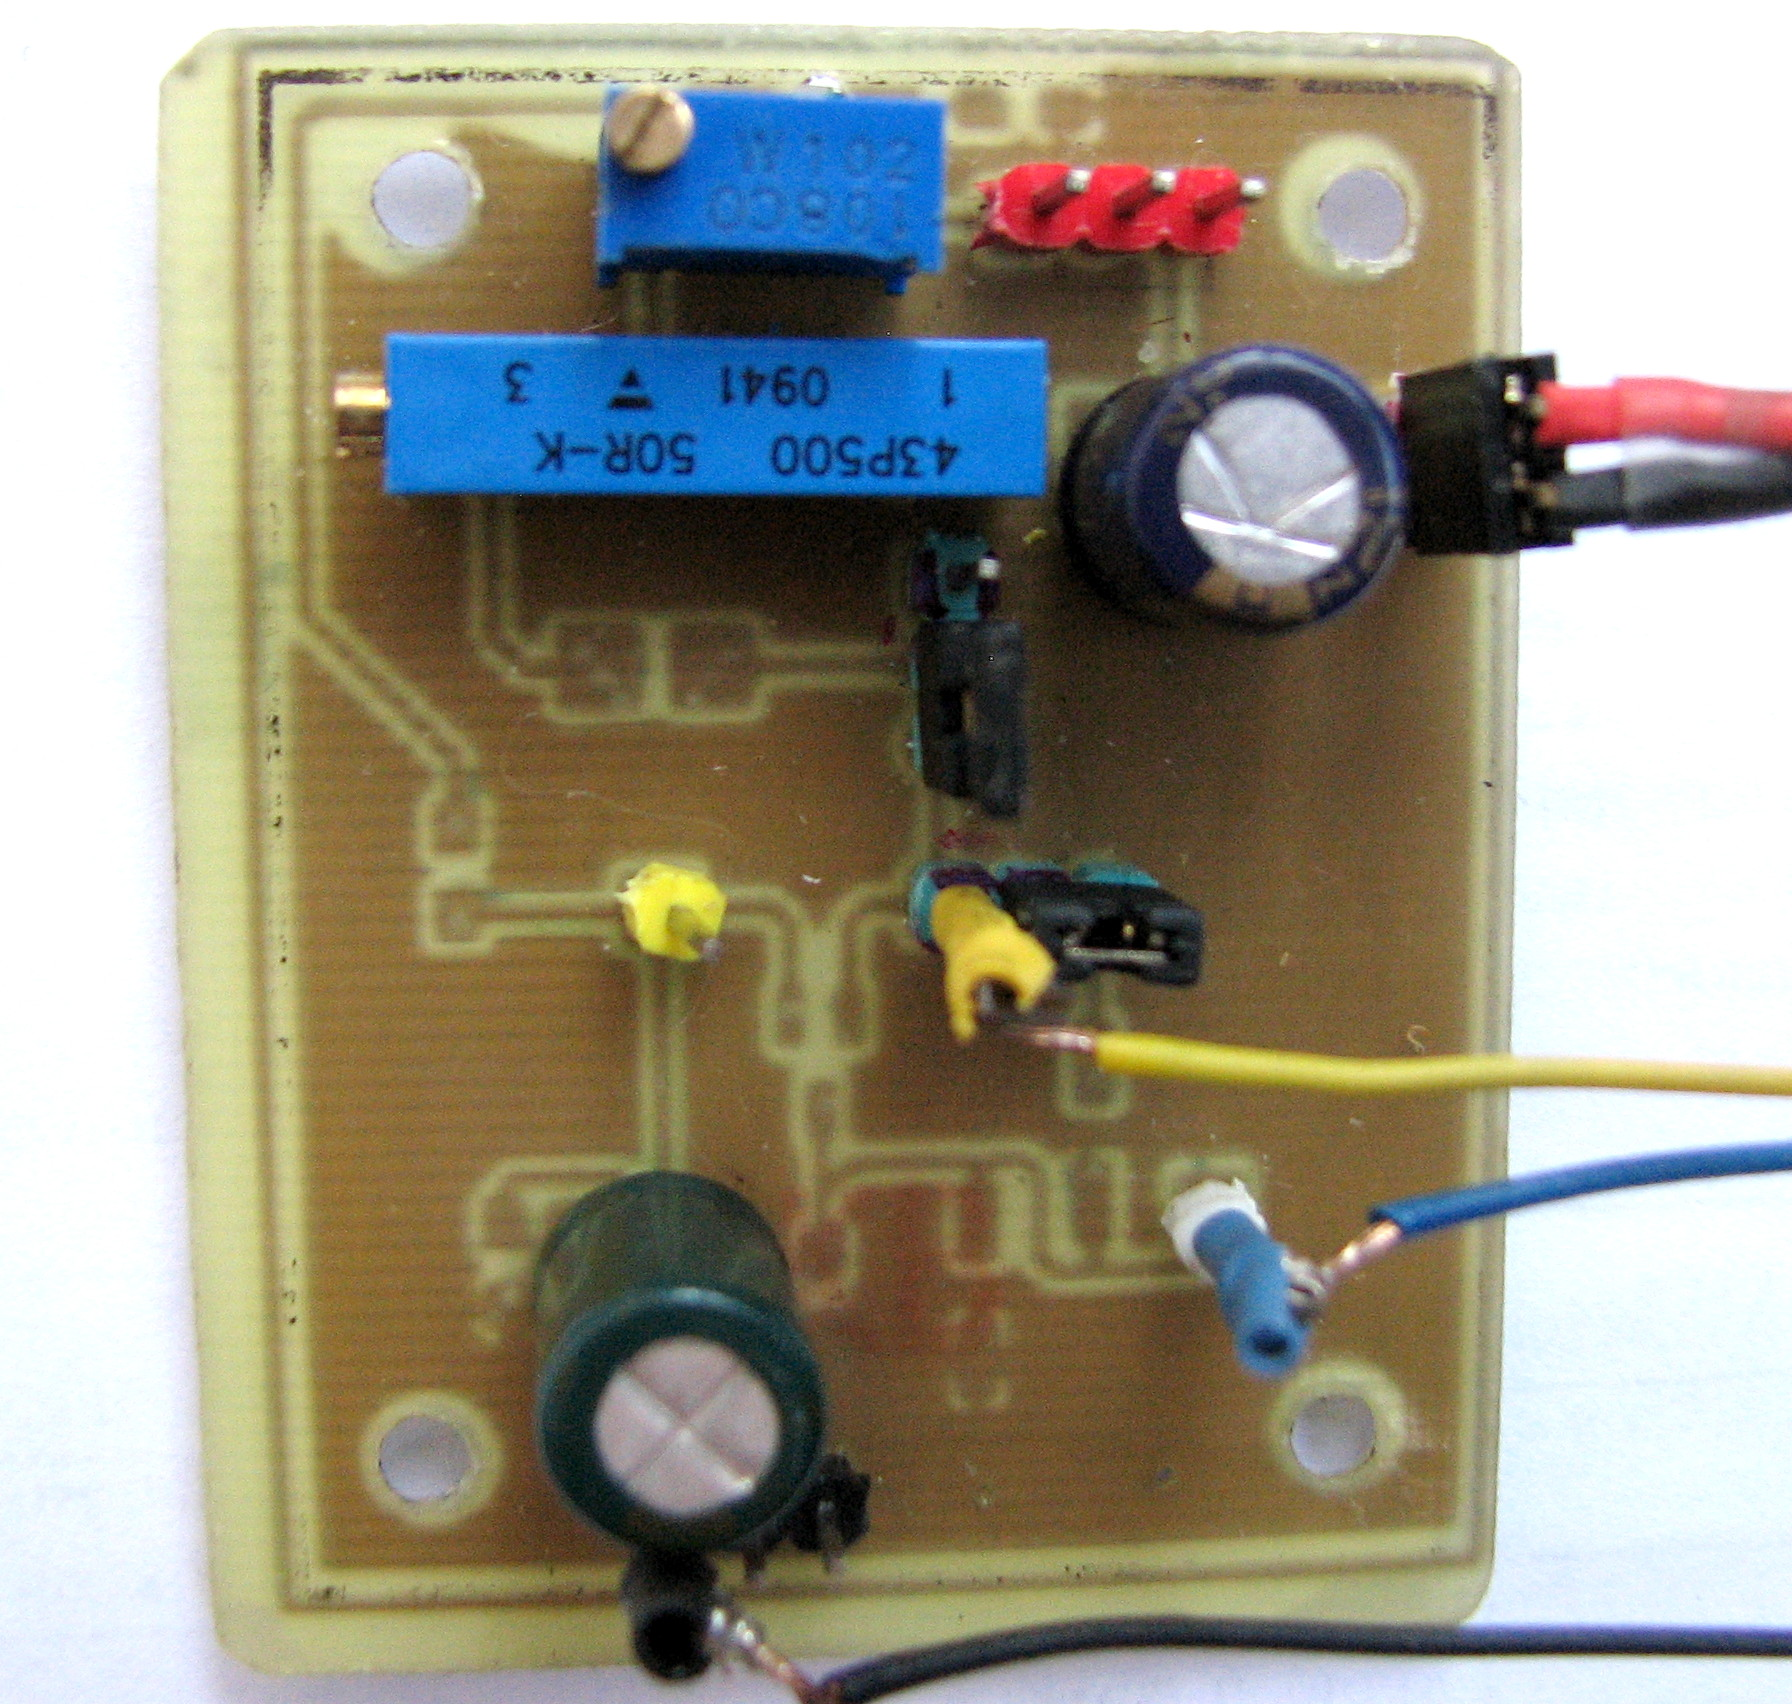
\includegraphics[width=0.5\textwidth]{p/colp_board.jpg} }
\caption{Печатная плата схемы генератора Колпитца}
\label{atu:f:colp_board}
\end{figure}


Описание дополнительных элементов.

Недостатки использования осцилла -- что вместо

Примеры динамики с сравнением.

\section{Численная модель генератора Колпитца}

Методы расчёта~\cite{zaeplnii_radio_calc}.

\section{Анализ и выбор критериев}

Проверяем старые.

Исследуем всякие.

\begin{figure}[htb!]
\centerline{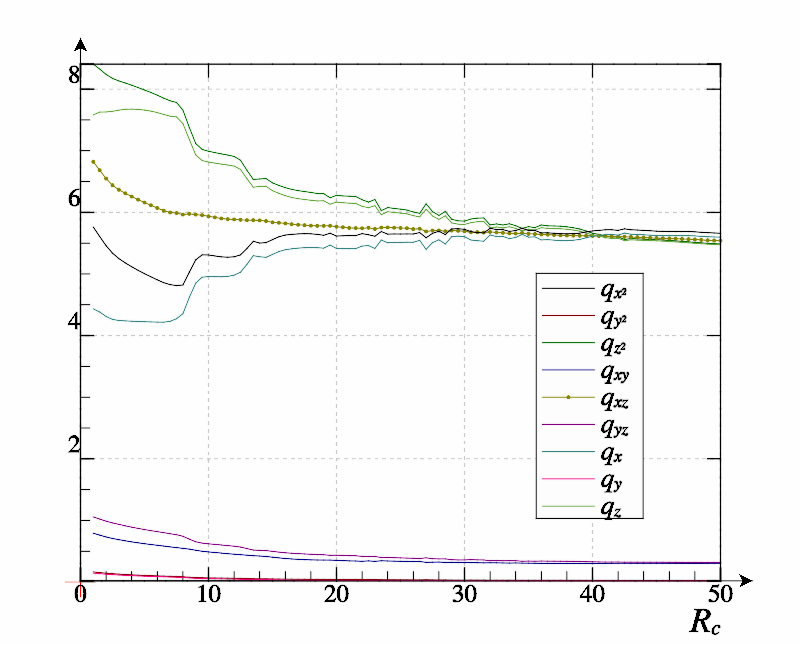
\includegraphics[width=0.7\textwidth]{p/colp_bjt_q-p_Rc_q.png} }
\caption{Зависимости значений критериев идентификации для модели системы Колпитца}
\label{atu:f:colp_bjt_q-p_Rc_q}
\end{figure}


\begin{figure}[htb!]
\centerline{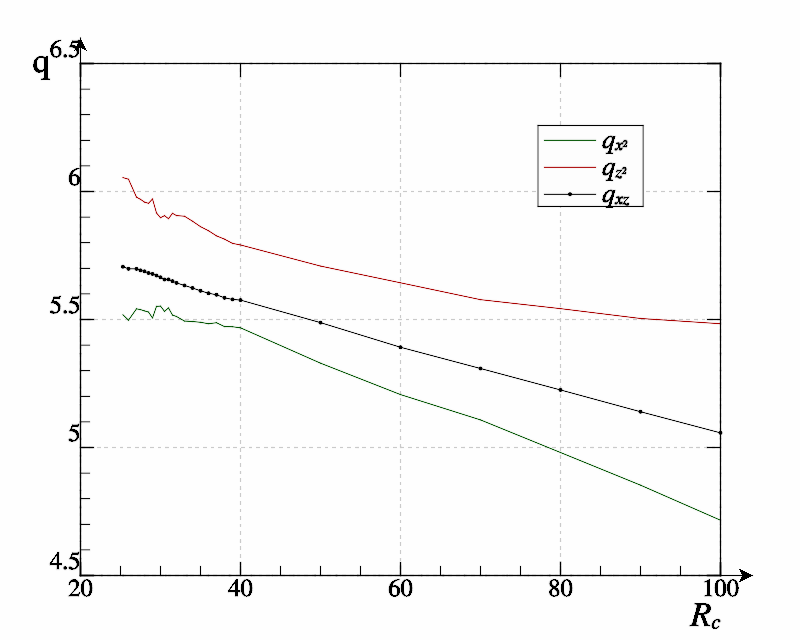
\includegraphics[width=0.7\textwidth]{p/colp_read_q-p_Rc_q.png} }
  \caption{Зависимости значений критериев идентификации $q_{x^2}$, $q_{z^2}$ и $q_{xz}$ для реального генератора Колпитца}
\label{atu:f:colp_read_q-p_Rc_q-p_Rc_q}
\end{figure}

\begin{figure}[htb!]
\centerline{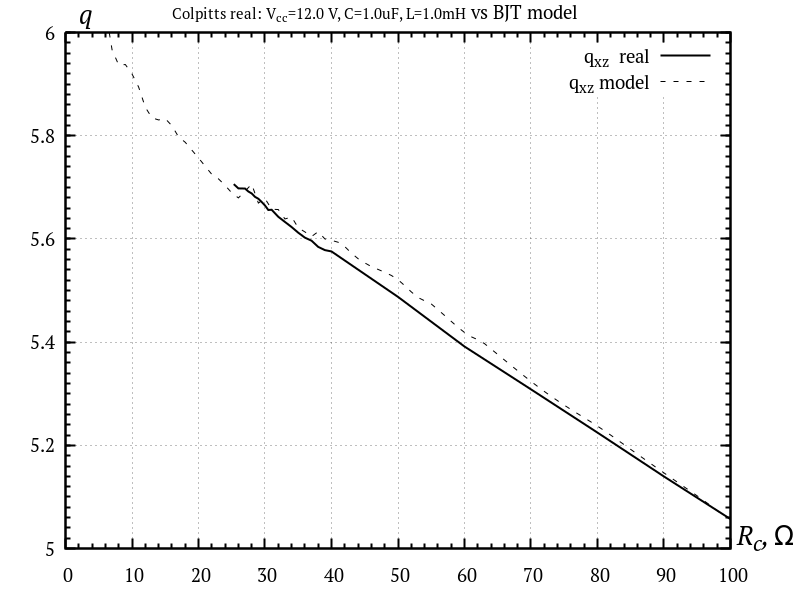
\includegraphics[width=0.7\textwidth]{p/colp_q_cml.png} }
\caption{Сравнение зависимостей значений критерия идентификации $q_{xz}$ реального генератора Колпитца с моделью}
\label{atu:f:colp_q_cml}
\end{figure}

Предлагаем новые.

\section{Синтез и анализ и системы идентификации}

Описание с картинкой.

Для процессов параметрической идентификации генератора Колпитца представлены результаты четырёх экспериментов,
проведённых в аналогичных условиях.

% C_1, C_2 = 1.0 uF, L = 1.0 mH, R_l=24.2 Ohm, R_e = 300 Ohm, R_1 = R_2 = 2.0 kOhm,
% Q: MMBT2222A: h_{FE}=210, V_{je} = 0.667V.
% V_{cc} = 12.0 V, V_{b} = 5.94 V
% d_0.txt: 27.3 - 44.2 Ohm  35.75 +-  8.45
% d_1.txt: 29.0 - 35.0 Ohm  32    +-  3
% d_2.txt: 26.0 - 30.0 Ohm  28    +-  2
% d_3.txt: 31.0 - 52.0 Ohm  41.5  +- 10.5
% d_4.txt: 29.0 - 32.0 Ohm  30.5  +-  1.5

Параметры первого эксперимента для генератора Колпитца
%
\begin{equation}
  \begin{array}{c}
    R_{c,\min} = \SI{27.3}{\ohm};
    \;
    R_{c,\max} = \SI{44.2}{\ohm};
    \;
    T_{R_c} = \SI{200}{\milli\second};
  \\
    R_c(t) = \SI{35.75}{\ohm} + \SI{8.45}{\ohm} \cdot \sin( \pi ( t + 1 ) ).
  \end{array}
  \label{atu:eq:colp_test1_cond}
\end{equation}

\begin{figure}[htb!]
  \centerline{
    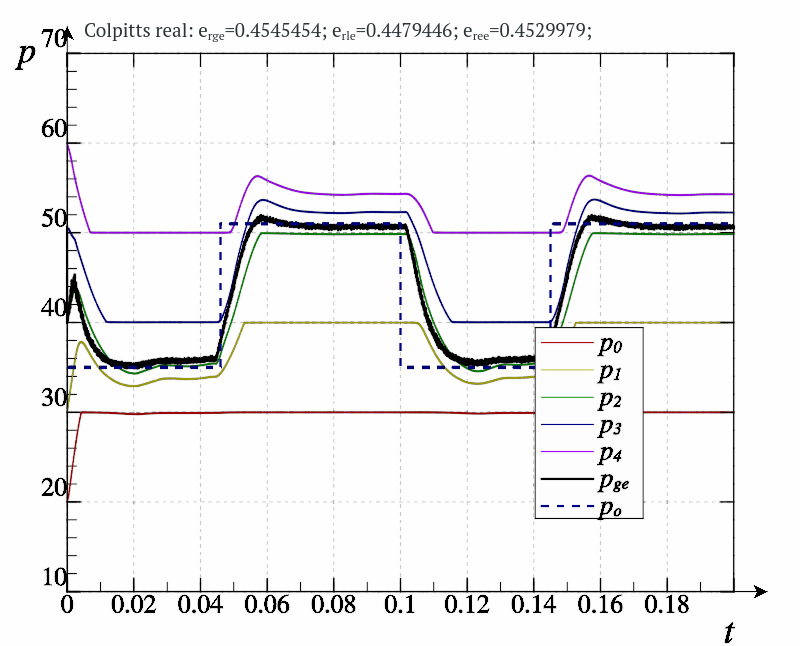
\includegraphics[width=0.48\textwidth]{p/colp_real_id_qi_fv5-p_p_01.png}
    \hfill
    \includegraphics[width=0.48\textwidth]{p/colp_real_id_qi_fv5-p_pp_01.png}
  }
  \caption{Процесс идентификации параметра $R_c$ реального генератора Колпитца '' при условиях }
  \label{atu:f:colp_r_id_1}
\end{figure}


Параметры второго эксперимента для генератора Колпитца
%
\begin{equation}
  \begin{array}{c}
    R_{c,\min} = \SI{29.0}{\ohm};
    \;
    R_{c,\max} = \SI{35.0}{\ohm};
    \;
    T_{R_c} = \SI{200}{\milli\second};
  \\
    R_c(t) = \SI{32.0}{\ohm} + \SI{3.0}{\ohm} \cdot \sin( \pi ( t + 1 ) ).
  \end{array}
  \label{atu:eq:colp_test2_cond}
\end{equation}

\begin{figure}[htb!]
  \centerline{
    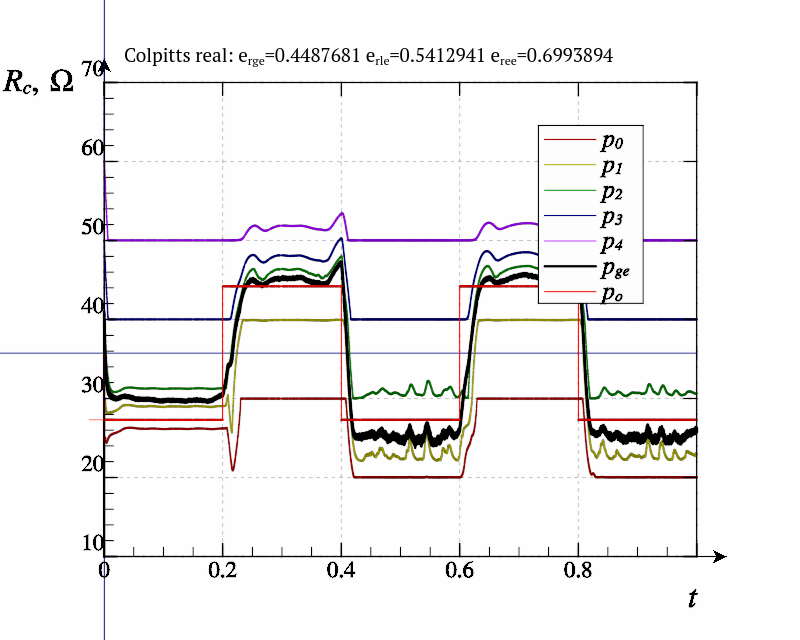
\includegraphics[width=0.48\textwidth]{p/colp_real_id_qi_fv5_0-p_p.png}
    \hfill
    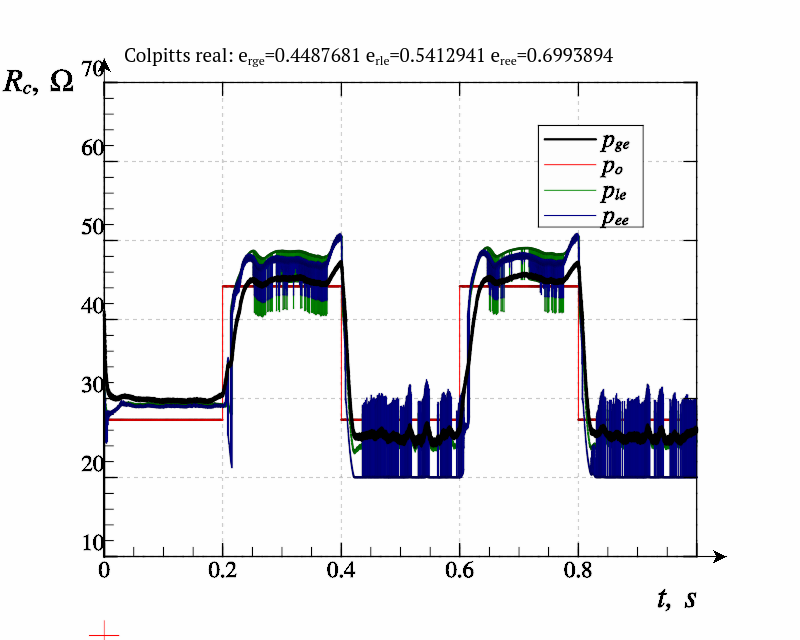
\includegraphics[width=0.48\textwidth]{p/colp_real_id_qi_fv5_0-p_pp.png}
  }
  \caption{Процесс идентификации системы  при условиях (первый эксперимент)}
  \label{atu:f:colp_real_id_qi_fv5_0}
\end{figure}

Параметры третьего эксперимента для генератора Колпитца
%
\begin{equation}
  \begin{array}{c}
    R_{c,\min} = \SI{31.0}{\ohm};
    \;
    R_{c,\max} = \SI{52.0}{\ohm};
    \;
    T_{R_c} = \SI{200}{\milli\second};
  \\
    R_c(t) = \SI{41.5}{\ohm} + \SI{10.5}{\ohm} \cdot \sin( \pi ( t + 1 ) ).
  \end{array}
  \label{atu:eq:colp_test3_cond}
\end{equation}

\begin{figure}[htb!]
  \centerline{
    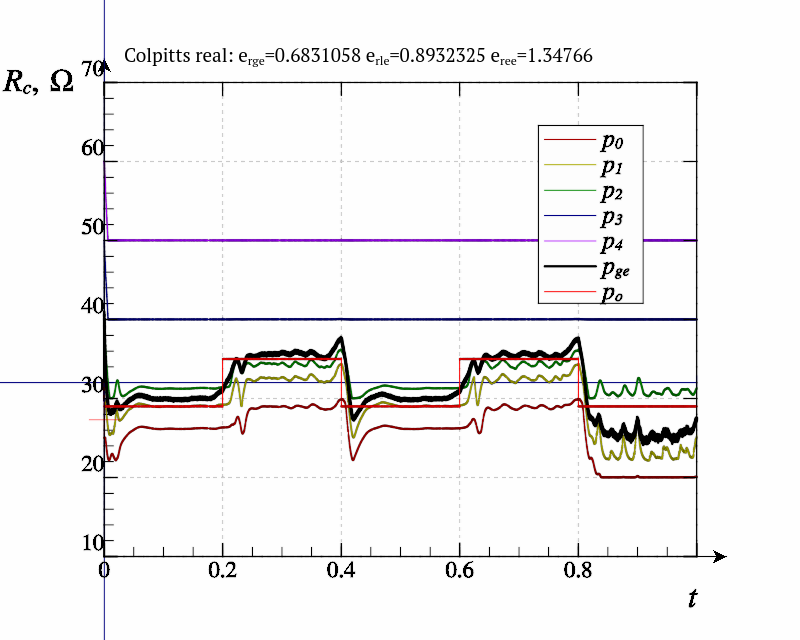
\includegraphics[width=0.48\textwidth]{p/colp_real_id_qi_fv5_1-p_p.png}
    \hfill
    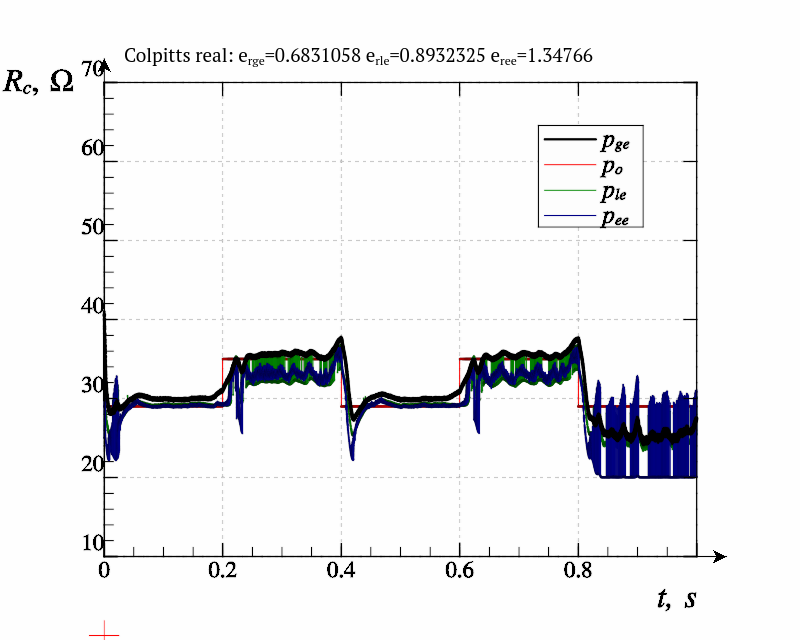
\includegraphics[width=0.48\textwidth]{p/colp_real_id_qi_fv5_1-p_pp.png}
  }
  \caption{Процесс идентификации системы  при условиях (второй эксперимент)}
  \label{atu:f:colp_real_id_qi_fv5_1}
\end{figure}


Параметры четвёртого эксперимента для генератора Колпитца
%
\begin{equation}
  \begin{array}{c}
    R_{c,\min} = \SI{29.0}{\ohm};
    \;
    R_{c,\max} = \SI{32.0}{\ohm};
    \;
    T_{R_c} = \SI{200}{\milli\second};
  \\
    R_c(t) = \SI{30.5}{\ohm} + \SI{1.5}{\ohm} \cdot \sin( \pi ( t + 1 ) ).
  \end{array}
  \label{atu:eq:colp_test4_cond}
\end{equation}

\begin{figure}[htb!]
  \centerline{
    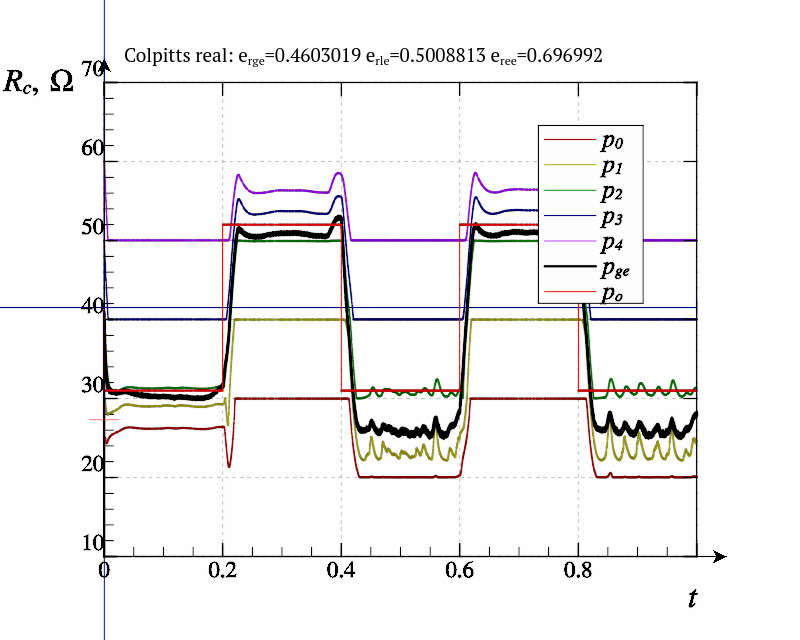
\includegraphics[width=0.48\textwidth]{p/colp_real_id_qi_fv5_3-p_p.png}
    \hfill
    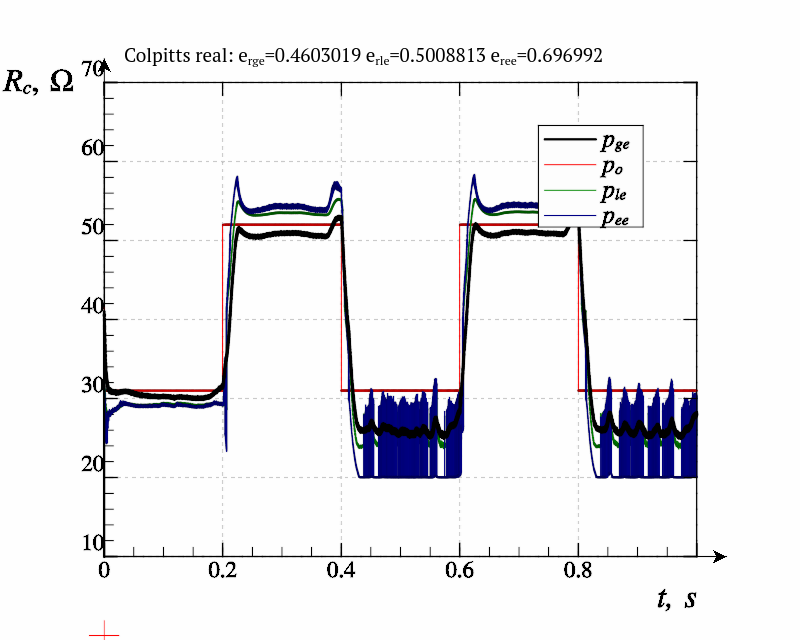
\includegraphics[width=0.48\textwidth]{p/colp_real_id_qi_fv5_3-p_pp.png}
  }
  \caption{Процесс идентификации системы  при условиях (третий эксперимент)}
  \label{atu:f:colp_real_id_qi_fv5_3}
\end{figure}


\begin{figure}[htb!]
  \centerline{
    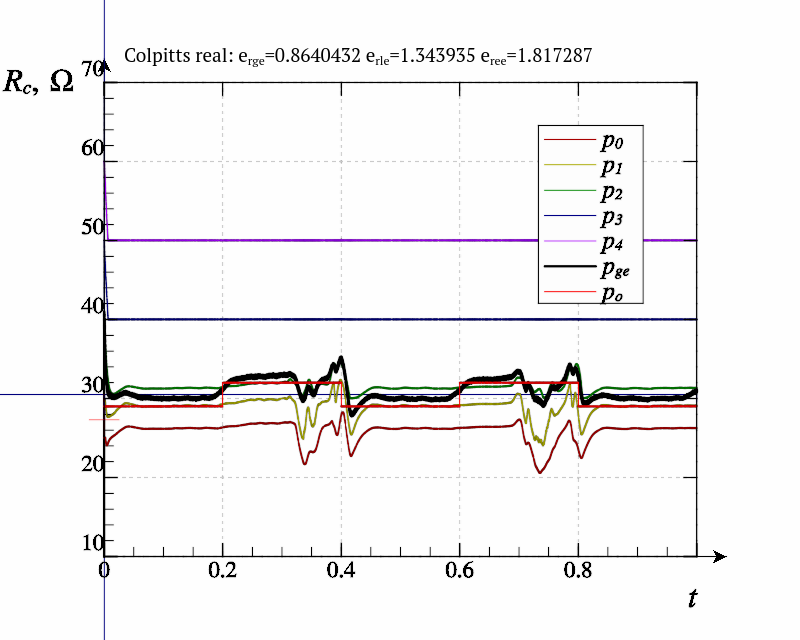
\includegraphics[width=0.48\textwidth]{p/colp_real_id_qi_fv5_4-p_p.png}
    \hfill
    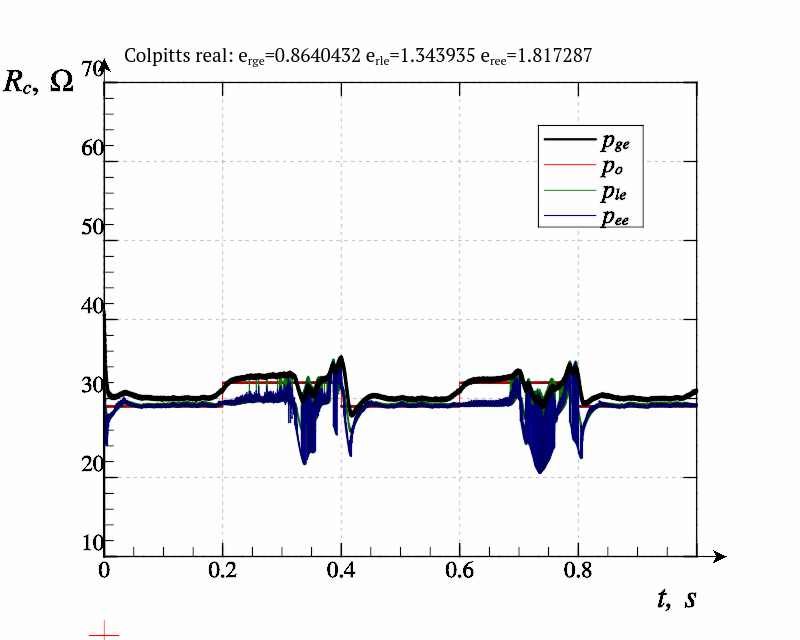
\includegraphics[width=0.48\textwidth]{p/colp_real_id_qi_fv5_4-p_pp.png}
  }
  \caption{Процесс идентификации системы  при условиях (четвёртый эксперимент)}
  \label{atu:f:colp_real_id_qi_fv5_4}
\end{figure}


Рассмотрим зависимости ошибок идентификации от параметров самой системы идентификации.
Параметр $a_q$, задающий
фильтрующие способности критерия идентификации, должен рассматриваться в первую очередь.
На рис.~\ref{atu:f:colp_real_id_qi_fv5_prm_0-p_a_q} представлены полученные зависимости
для процессов идентификации параметра $R_c$ генератора Колпитца.

\begin{figure}[htb!]
  \centerline{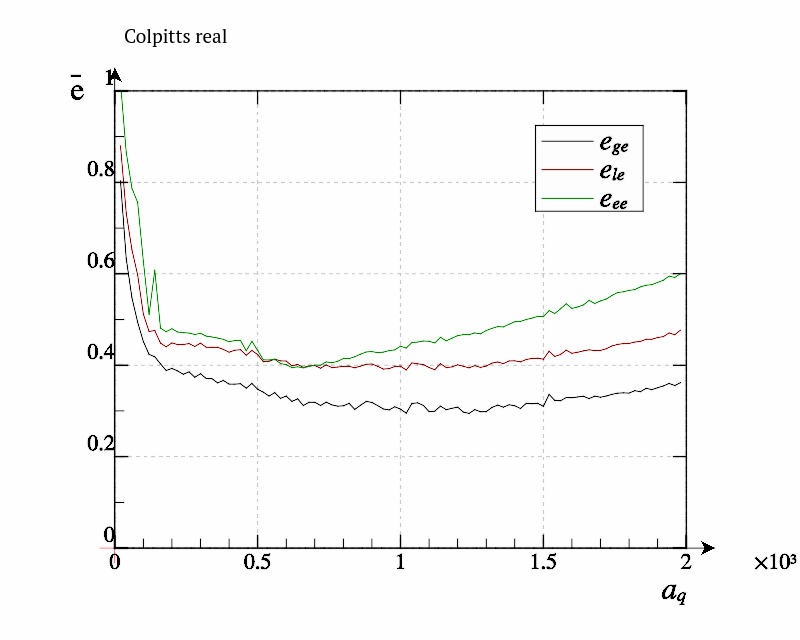
\includegraphics[width=0.6\textwidth]{p/colp_real_id_qi_fv5_prm_0-p_a_q.png} }
  \caption{Зависимости $\overline{e}_{r*}(a_q)$ при идентификации параметра $R_c$ генератора Колпитца}
  \label{atu:f:colp_real_id_qi_fv5_prm_0-p_a_q}
\end{figure}


\begin{figure}[htb!]
  \centerline{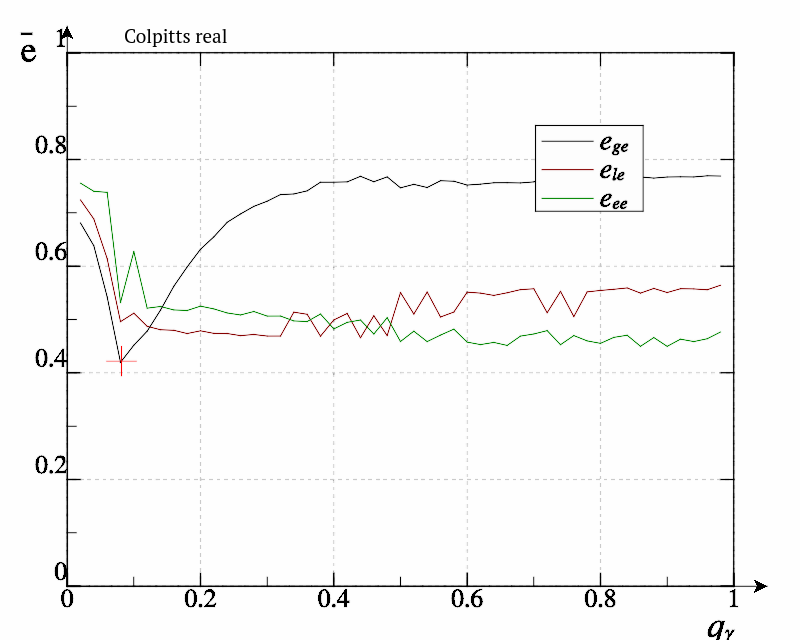
\includegraphics[width=0.6\textwidth]{p/colp_real_id_qi_fv5_prm_0-p_q_gamma.png} }
  \caption{Зависимости $\overline{e}_{r*}(q_\gamma)$ при идентификации параметра $R_c$ генератора Колпитца}
  \label{atu:f:colp_real_id_qi_fv5_prm_0-p_q_gamma}
\end{figure}

\begin{figure}[htb!]
  \centerline{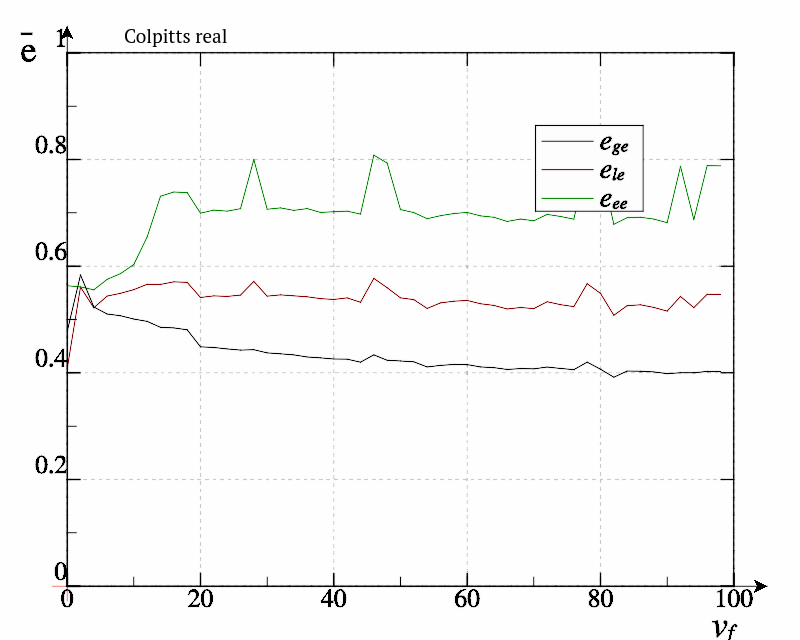
\includegraphics[width=0.6\textwidth]{p/colp_real_id_qi_fv5_prm_0-p_v_f.png} }
  \caption{Зависимости $\overline{e}_{r*}(v_f)$ при идентификации параметра $R_c$ генератора Колпитца}
  \label{atu:f:colp_real_id_qi_fv5_prm_0-p_v_f}
\end{figure}


\begin{figure}[htb!]
  \centerline{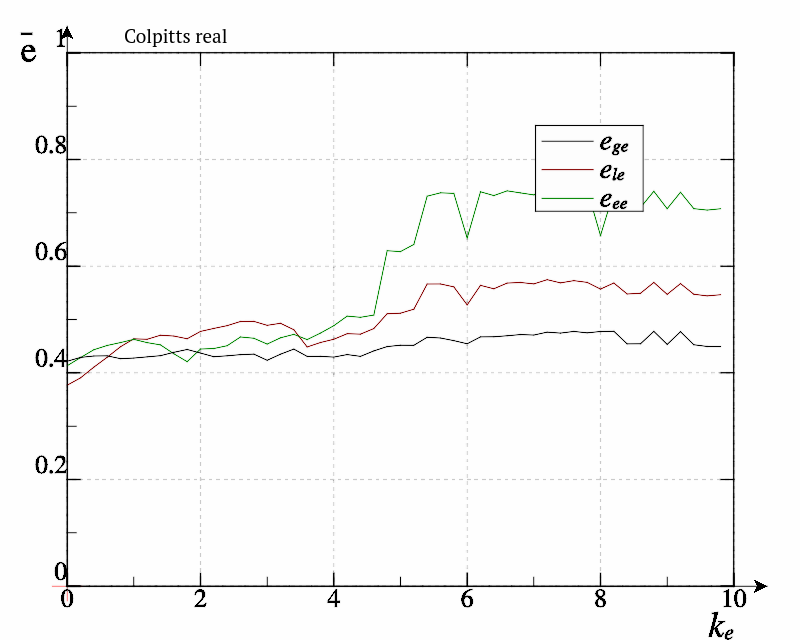
\includegraphics[width=0.6\textwidth]{p/colp_real_id_qi_fv5_prm_0-p_k_e.png} }
  \caption{Зависимости $\overline{e}_{r*}(k_e)$ при идентификации параметра $R_c$ генератора Колпитца}
  \label{atu:f:colp_real_id_qi_fv5_prm_0-p_k_e}
\end{figure}


\begin{figure}[htb!]
  \centerline{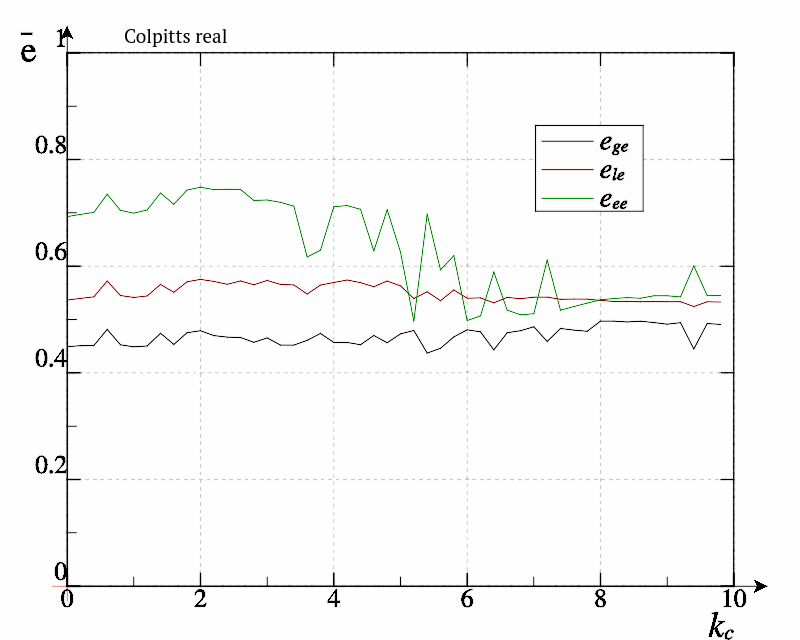
\includegraphics[width=0.6\textwidth]{p/colp_real_id_qi_fv5_prm_0-p_k_cl.png} }
  \caption{Зависимости $\overline{e}_{r*}(k_c)$ при идентификации параметра $R_c$ генератора Колпитца}
  \label{atu:f:colp_real_id_qi_fv5_prm_0-p_k_cl}
\end{figure}


\begin{figure}[htb!]
  \centerline{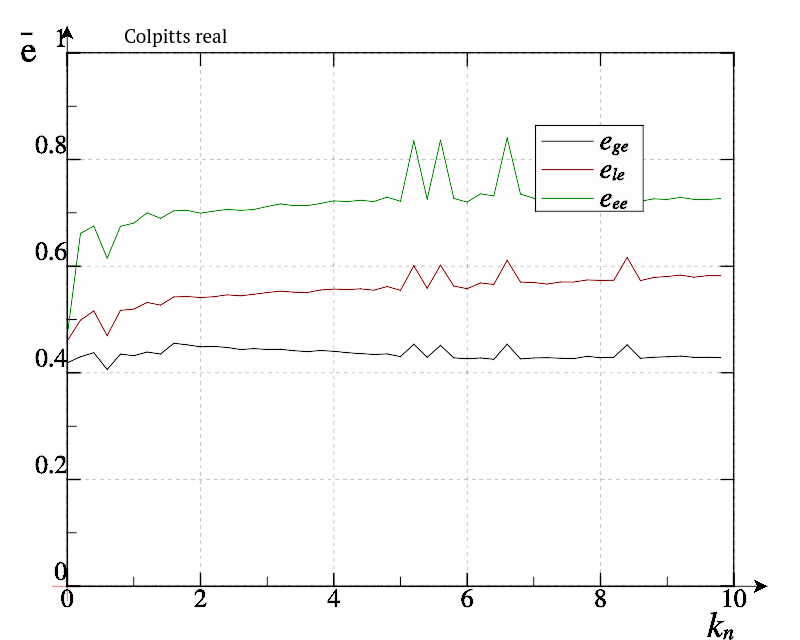
\includegraphics[width=0.6\textwidth]{p/colp_real_id_qi_fv5_prm_0-p_k_cn.png} }
  \caption{Зависимости $\overline{e}_{r*}(c_n)$ при идентификации параметра $R_c$ генератора Колпитца}
  \label{atu:f:colp_real_id_qi_fv5_prm_0-p_k_cn.png}
\end{figure}



\section{Выводы по разделу \thechapter}

Выводы.

